\chapter{Analysis}

%---------------------------------------------------------------
\section{Static Typing in JavaScript}
%---------------------------------------------------------------

JavaScript is a dynamically typed programming language, where users do not need to assign types to a variable or a function and the type is inferred automatically by the JavaScript engine. This is a great feature of JavaScript, which lowers the barrier of entry to writing JavaScript code and allows developers to prototype and write code quickly, proven by the growth of popularity of JavaScript in the last decade, making it the most commonly used programming language according to the 2022 Stack Overflow Developer Survey \cite{StackOverflowDeveloper}.

However, dynamic typing has its drawbacks, as it is harder to spot trivial errors in the code without running it beforehand and it is more difficult to refactor the code without breaking it, which often leads to poor software quality \cite{fardJSNOSEDetectingJavaScript2013a}. Proponents of static typing insist that static types allow developers to spot potential bugs and mistakes earlier during development and that it allows for better tooling, such as more rich code completion and refactoring tools.

There is an upcoming TC39 proposal for adding type annotations, broadly inspired by TypeScript syntax \cite{ECMAScriptProposalType2023}. These annotations are only useful for build-time tooling as they are ignored in runtime. The proposal suggests that these annotations should be erased by an additional compilation step. Even though users can already provide static types using JSDoc right now, the syntax is not as clean as the proposed TypeScript-like syntax.

Regardless, many languages aim to introduce static typing to JavaScript, such as Flow or TypeScript, or alternative languages which compile back to JavaScript, such as Elm or ReScript.

\subsection{Elm}

Elm is a functional programming language designed specifically for building web applications \cite{ElmDelightfulLanguage}. The language compiles to JavaScript and has a strong static Hindley-Milner-based type system, which allows inferring types more often and reliably. Elm does not provide any escape hatches such as \code|any| in TypeScript, thus it is harder to write unsafe code, as the types must be valid for the code to be compiled.

Elm also includes a lot of quality-of-life improvements and benefits, for instance: enforced purity of functions, out-of-the-box immutability, \code|case| pattern matching, JSON decoders and encoders for strict parsing, \code|Maybe| and \code|Result| monads for avoiding \code|null| and \code|undefined| references or its own virtual DOM implementation for efficient rendering of interactive user interfaces. Notably, the Elm Architecture, where the application code is organized into three parts: model, update and view \cite{ElmArchitectureIntroduction}, has greatly inspired other libraries and frameworks like Redux \cite{PriorArtRedux2022}.

\subsection{ReScript}

ReScript is a programming language built on top of the OCaml toolchain. Unlike Flow or TypeScript, ReScript is not a superset of JavaScript, instead, the language compiles to JavaScript. ReScript was created as a spin-off from the Reason programming language and accompanying BuckleScript compiler, aiming to vertically integrate and streamline the adoption barrier caused by the need to be familiar with multiple unrelated tools and toolchains \cite{BuckleScriptReasonRebranding}.

The language aims to be more sound with more powerful type inference than TypeScript, borrowing the Hindler-Milner type system from OCaml implementation \cite{EfficientInsightfulGeneralization,HistoryReScript2022}, thus most of time the types can be inferred automatically without the need to annotate them explicitly, whereas TypeScript utilizes bidirectional type checking \cite{ReconstructingTypeScriptPart}.

\subsection{Flow}

Flow is a static type checker for JavaScript \cite{chaudhuriFastPreciseType2017,Flow2023}, which allows developers to annotate their code with static types. Flow is developed by Meta and is internally used in production by Facebook, Instagram and React Native. Type annotations in Flow are fully eraseable, which means that the type annotations can be fully removed from the Flow code to emit valid JavaScript code. The checking of these types is occurring at compile-time before removal in build-time. Flow is also a superset of JavaScript, which means any JavaScript code is a valid Flow code.

One of the primary goals of Flow is to provide type soundness; the ability to catch every error that might happen in runtime at compile-time, no matter how likely it is to happen. This means, that a valid Flow code can provide developers some guarantees about the type a value has in runtime, at the expense of catching errors, which are unlikely to happen in runtime.

Both Flow and TypeScript are similar regarding features at the time of writing. Most of the soundness differences between Flow and TypeScript have been addressed with the newer versions of TypeScript, even though soundness is a specific non-goal by the TypeScript team \cite{TypeScriptDesignGoals}. However, developers must opt-in to these features by setting \code|"strict"| to \code|"true"| in \code|tsconfig.json|, whereas in Flow these features are enabled by default.

\subsection{TypeScript}

TypeScript is a statically typed programming language developed and maintained by Microsoft \cite{TypeScriptJavaScriptSyntax}. It is a language that compiles down to JavaScript and adds static type checking to JavaScript \cite{DocumentationTypeScriptJavaScript}. Unlike Elm or ReScript, TypeScript is a syntactical superset of JavaScript, which means that any valid JavaScript code can be a valid TypeScript code\footnote{With a lax compiler configuration}. Similar to Flow, type annotations provided by the developer are fully erasable either by the TypeScript \code|tsc| compiler or by other community build tools, such as \code|babel|\cite{BabelCompilerNext}, \code|esbuild|\cite{EsbuildExtremelyFast} or \code|swc|\cite{SWCRustbasedPlatform}.

Type system in TypeScript is considered to be less sound and more forgiving, as soundness is stated as an explicit non-goal for the design team of TypeScript \cite{TypeScriptDesignGoals}, with emphasis on striking a balance between productivity and correctness. By default, the TypeScript compiler is not strict and the language itself includes an escape hatch for developers to opt out of type checking by using the \code|any| type or using \code|@ts-ignore| comment annotations. Nevertheless, with proper compiler configuration, the type system of TypeScript can be as sound as in Flow.

Both Flow and TypeScript support advanced features such as generics and utility types, with the latter supporting template string literal types and better support for conditional types, unlocking the potential of writing more expressive types, which this master thesis will further explore in more detail.

TypeScript has become the de-facto standard for writing JavaScript code with static types. With deep integration with Visual Studio Code \cite{VisualStudioCode}, the rich build ecosystem and high compatibility with existing JavaScript libraries and tools, TypeScript has become one of the fastest growing languages in terms of usage according to the 2022 Octoverse report by Github \cite{Octoverse2022State}.

\section{Typescript syntax}

Typescript adds optional static types to JavaScript, which can be applied to add constraints to code constructs such as functions, variables and properties, so that compilers, linters and other development tools can provide better and useful insights during software development \cite{hejlsbergTypeScriptLanguageSpecification}.

Types in TypeScript can be categorized into primitive types, literal types, data structure types, union types, intersection types and type parameters. All of these types introduce static constraints on their values.

A primitive value is data, that is not an object and has no methods or properties. These primitives are immutable, thus they cannot be altered. Similar to JavaScript, TypeScript has the following types of primitive values:

\begin{listing}[h]
  \caption{Primitive Types}
  \begin{minted}{TypeScript}
type Primitive = 
  | string | number | bigint
  | boolean | undefined | symbol | null;
\end{minted}
\end{listing}

Some primitive values represent a singular data value, such as \code{null} or \code{undefined}, but many of these primitives can represent an infinite number of values, like \code{number}, \code{bignumber} or \code{string}.

Literal types are a subset of primitive values, which are used to describe an exact possible value.

\begin{listing}[h]
  \caption{Literal Types}
  \begin{minted}{TypeScript}
type Literal = "foo" | 42 | true | 100n;
\end{minted}
\end{listing}

To represent data structures such as objects and arrays, we can use the following types: objects, records, tuples and arrays.

\begin{listing}[h]
  \caption{Data structures}
  \begin{minted}{TypeScript}
type Structures = 
  | { foo: string, bar: number }     // object
  | { [key in keyof Keys]: number }  // record
  | [number, string]                 // tuple
  | number[]                         // array
\end{minted}
\end{listing}

TypeScript uses structured typing, which means that TypeScript only validates the shape of the data. Essentially, if the data has the same shape as the type, it is considered to be of that type. This is also known as duck typing, essentially if it walks like a duck and quacks like a duck, it is a duck.

\begin{listing}[h]
  \caption{Duck typing}
  \begin{minted}{TypeScript}
type DuckLike = { quack: () => void; type: string };

const Duck: DuckLike = {
  quack: () => console.log("duck!"),
  type: "duck",
};

// this will be still valid
const Goose: DuckLike = {
  quack: () => console.log("goose!"),
  type: "goose",
};
\end{minted}
\end{listing}

Structured typing does include some drawbacks unlike in nominal type systems, where each type is unique and the same data cannot be assigned across types, but these can be easily mitigated using literal types to act as brands.

\begin{listing}[h]
  \caption{Nominal typing in TS}
  \begin{minted}{TypeScript}
type DuckLike = { quack: () => void; type: "duck" };

const Duck: DuckLike = {
  quack: () => console.log("duck!"),
  type: "duck",
};

// this will not be valid
const Goose: DuckLike = {
  quack: () => console.log("goose!"),
  type: "goose",
};
\end{minted}
\end{listing}


Types can be generalized into sets, where each type can contain a set of values. A type can be a subset or a superset of another type.

\begin{figure}[h]
  \centering
  \resizebox{0.7\textwidth}{!}{
    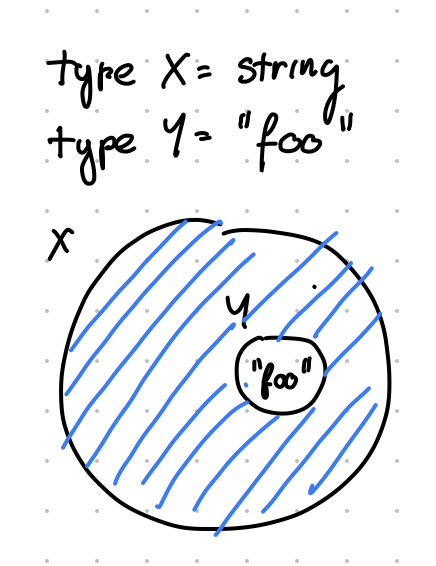
\includegraphics{text/analysis/2023-03-21-20-08-52.png}
  }
  \caption{~Types represented as sets}
\end{figure}

Similar to other sets in mathematics, types can be combined using unions. With unions, we can broaden the scope of the type to represent multiple values.

\begin{figure}[h]
  \centering
  \resizebox{\textwidth}{!}{
    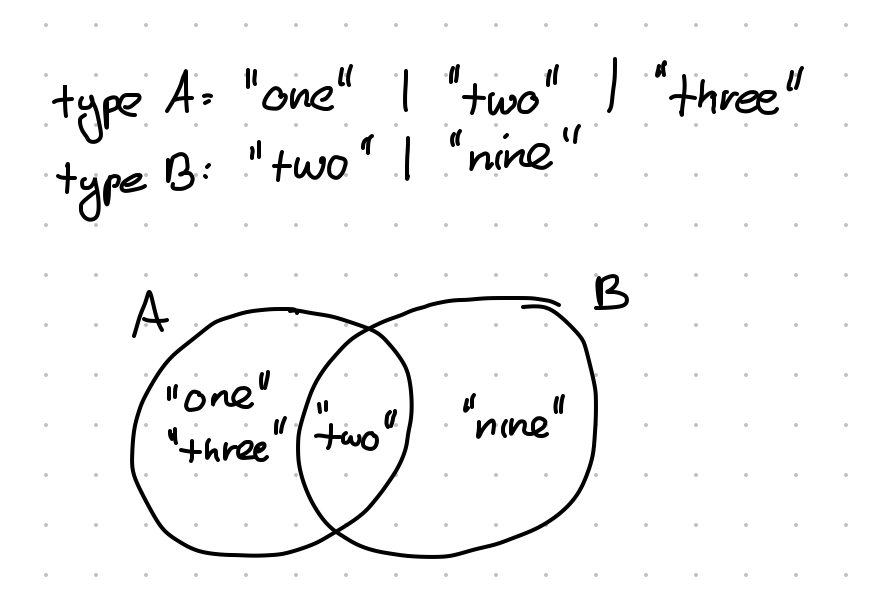
\includegraphics{text/analysis/2023-03-21-20-00-30.png}
  }
  \caption{~Union of types}
\end{figure}

Types can also intersect each other to create a narrower type.

\todo{type intersection}

TypeScript includes two top types, also known as universal types or supertypes: \code{any} and \code{unknown}. These types are used to represent any possible value.

\code{any} is a top type, where every type is assignable to type \code{any} and type \code{any} is assignable to every type \cite{TopTypesAny}. \code{any} is acting as an escape hatch to opt out of type checking. This does have unintended consequences, especially when dealing with external data, most notably when the return type of \code{JSON.parse()} and \code{Response.json()} is \code{any}. As \code{any} is assignable to every type, it can be assigned to a different type without any warnings.

\todo{Add any code example}

\code{unknown} acts as a more restrictive version of \code{any}. Every type is assignable to type \code{unknown}, but \code{unknown} is not assignable to any other type. To assign \code{unknown} to a different type, we must narrow the types using either type guards, type assertions, equality checks or other assertion functions.

\todo{Add unknown code example}

\code{never} is a bottom type, acting as a subtype of all other types, representing a value that should never occur. In the context of the theory of mathematical logic, \code{never} acts as a logical contradiction, describing a value that may never exist, which is especially useful to model stop gaps within type-level functions. No other type can be assigned to \code{never} nor \code{never} cannot be assigned to any other type.

\todo{Add unknown code example}

\code{enum} type is a distinct subtype used to describe a set of named constants. Instead of using individual variables for each constant, an \code{enum} provides an organized way to express a collection of related values. \code{enum} is one of the few TypeScript features which introduce an additional code added to the compiler output and enums refer to real objects at runtime.

An \code{enum} type consists of members and their corresponding initializers for the runtime value of the member. There are two types of enums in TypeScript: numeric enums and string-based enums:

\begin{listing}[h]
  \caption{Numeric enums}
  \begin{minted}{TypeScript}
enum Direction {
  Up = 1,
  Down,
  Left,
  Right,
}
\end{minted}
\end{listing}

In numeric enums, each member is assigned a numeric literal value. Each member can have an optional initializer to specify an exact number corresponding to a member. If omitted, the value of the member will be generated by auto-incrementing from previous members.

String-based enums are similar in nature, where each member is assigned a string literal value instead. Each member thus must have an initializer with a string literal. The key benefit of string-based enums is that they tend to keep their semantic value well when serializing, which is especially helpful when debugging, as the values of numeric enums tend to be opaque.

\begin{listing}[h]
  \caption{Numeric enums}
  \begin{minted}{TypeScript}
enum Direction {
  Up = "UP",
  Down = "DOWN",
  Left = "LEFT",
  Right = "RIGHT",
}
\end{minted}
\end{listing}

Functions and \code{void}

Void
\todo{Enums}

Arrays

\code{any}, \code{never}, \code{unknown}

Object

Generics

\begin{itemize}
  \item Terminology - generics, type arguments, return type
  \item Conditional types
  \item Recursive types
  \item Mapped types
  \item Template Literal Types
\end{itemize}

\subsection{Types and their assignability}

\begin{itemize}
  \item Primitive Types
  \item Literal Types
  \item \code{unknown}, \code{never}, \code{any}
  \item Structures (nominal vs structural typing)
  \item Unions and Intersections
\end{itemize}

\subsection{Conditional Types}
\subsection{Conditional Types}
\subsection{Recursive Types}
\subsection{Mapped Types}
\subsection{Template Literal Types}

\section{Prior Art}

\begin{itemize}
  \item \code{kawayiLinLin/typescript-lodash}
  \item \code{arielhs/ts-arithmetic}
  \item \code{ts-belt}
  \item \code{type-fest}
\end{itemize}